% !TeX root = ../main.tex

\chapter{Preliminaries}
\label{ch:preliminaries}

\section{Notations}
In this section, we present the notations used throughout this thesis, as listed below:

\begin{table}[H]
    \centering
    \begin{tabular}{ |p{2cm}||p{10cm}|  }
    % \begin{tabular}{ |c|l| }
        \hline
        Notation  & Definition\\
         \hline
         $\ket{0}, \ket{1}$ & They are the two computational basis states of a single qubit, represented as orthonormal column vectors in a 2-dimensional complex Hilbert space $\mathbb{C}^{2}$ that $$\ket{0} = \begin{pmatrix}1 \\ 0\end{pmatrix}, \ket{1} = \begin{pmatrix}0 \\ 1\end{pmatrix}$$\\
         \hline
         $\dagger$ & The dagger operation transposes the Pauli matrix and then takes its complex conjugate.\\
         \hline
         $\mathbb{F}_{2}$ & The finite field with two elements $\{0, 1\}$, where addition and multiplication are performed modulo 2. \\
         \hline
         $\oplus$ & The XOR computation in logic representation.\\
         \hline
         $I_{n}$ & The $n \times n$ identity matrix over $\mathbb{F}_{2}$.\\
         \hline
         $GF(2^{n})$, $GF(n, \mathbb{F}_{2})$ & The finite field with $2^{n}$ elements, the unique finite field of characteristic 2 and order $2^{n}$, constructed as a degree-$n$ extension of $\mathbb{F}_{2}$.\\
         \hline
         $GL(n, \mathbb{F}_{2})$ & The general linear group of degree $n$ over $\mathbb{F}_{2}$, the group of all invertible $n \times n$ matrices with entries in $\mathbb{F}_{2}$, under matrix multiplication.\\
    \hline
\end{tabular}
    \caption{Some notations used in this paper}
    \label{tab:Notations}
\end{table}



\section{Quantum Circuits}
From the Enigma machine to computers based on the von Neumann architecture, 
all of these systems consist of wires and logic gates that execute their 
operations. Quantum computers are constructed from analogous components, 
combining quantum wires and quantum logic gates to form quantum circuits, 
which carry quantum bits and execute algorithms.

These are the flesh and blood of quantum computers, and we use these elements to describe the superposition state through Dirac notation:


\begin{equation}
    \ket{\psi} = \alpha\ket{0} + \beta\ket{1}
\end{equation}

In this section, we introduce some fundamental elements of quantum circuits, including the NOT and Controlled-NOT gates. These gates can be understood through matrix operations, and circuits constructed using only these gates are referred to as CNOT-based circuits.

Since gate-level circuits are the most commonly used construction today, we focus our efforts on reducing them.

First, consider the NOT gate, or, in terms of the Pauli matrices, the $X$ gate. Its operation can be defined by its truth table: from a classical perspective, it maps the input bit $0 \rightarrow 1$ and $1 \rightarrow 0$. From a quantum perspective, however, we instead take the inputs as $\ket{0}$ and $\ket{1}$, and the gate acts linearly on $\ket{\psi}$. Through the matrix $X$, the state changes as follows:

\begin{figure}[htbp]
\centering
\begin{minipage}{0.45\textwidth}
\centering
\begin{displaymath}
\begin{array}{c|c}
\hline
a & \bar{a} \\
\hline
0 & 1  \\
1 & 0  \\
\end{array}
\end{displaymath}
\end{minipage}%
\hfill
\begin{minipage}{0.45\textwidth}
\centering
\[
X \equiv \begin{bmatrix} 0 & 1 \\ 1 & 0 \end{bmatrix}
\]
\end{minipage}
\caption{The left-hand side shows the truth table for the NOT gate, while the right-hand side shows the Pauli-$X$ matrix, reflecting the quantum perspective of the NOT gate.}
\label{fig:not-truth-table-and-pauli-x}
\end{figure}

\begin{figure}[htbp]
\centering
\begin{minipage}{0.45\textwidth}
\centering
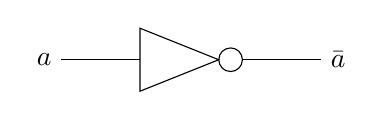
\begin{tikzpicture}
  % input wire
  \draw (0,0) -- (1,0);
  % NOT gate body (triangle)
  \draw (1,0.4) -- (1,-0.4) -- (2,0) -- cycle;
  % bubble (inversion circle)
  \draw (2.15,0) circle (0.15);
  % output wire
  \draw (2.3,0) -- (3.3,0);
  % labels
  \node[left] at (0,0) {$a$};
  \node[right] at (3.3,0) {$\bar{a}$};
\end{tikzpicture}
\end{minipage}%
\hfill
\begin{minipage}{0.45\textwidth}
\centering
\begin{quantikz}
\lstick{$\ket{a}$} & \gate{X} & \rstick{$\ket{a \oplus 1}$} \qw
\end{quantikz}
\end{minipage}
\caption{The left-hand side shows the classical NOT logic gate, while the right-hand side shows the quantum Pauli-X gate.}
\label{fig:NOT-gate}
\end{figure}

We can also represent the state as a column vector, $\begin{bmatrix} \alpha \\ \beta \end{bmatrix}$, such that

\begin{equation}
    X\begin{bmatrix}\alpha \\ \beta\end{bmatrix} = \begin{bmatrix}\beta \\ \alpha\end{bmatrix}
\end{equation}

This is a single-qubit gate that also satisfies the \textbf{unitary} property, meaning $X^{\dagger}X \equiv I$. It transforms the input state $\alpha\ket{0} + \beta\ket{1}$ into $\alpha\ket{1} + \beta\ket{0}$, where the normalization condition $|\alpha|^{2} + |\beta|^{2} = 1$ is preserved.

Next, to operate on two qubits and achieve a generalized XOR operation, the Controlled-NOT gate, or CNOT gate, is required. The exclusive-OR is a remarkably useful operator: it diffuses bit-streams efficiently in classical computation, and likewise provides an efficient means of executing and transferring information in quantum circuits. This multi-qubit quantum logic gate has two inputs, one serving as the control, on the top line, and the other as the target, on the bottom line.

\begin{figure}[htbp]
\centering
\begin{minipage}{0.45\textwidth}
\centering
\begin{displaymath}
\begin{array}{c|c}
\hline
{\ket{ab}} & {\ket{a'b'}}\\
\hline
{\ket{00}} & {\ket{00}}  \\
{\ket{01}} & {\ket{01}}  \\
{\ket{10}} & {\ket{11}}  \\
{\ket{11}} & {\ket{10}}  \\
\end{array}
\end{displaymath}
\end{minipage}%
\hfill
\begin{minipage}{0.45\textwidth}
\centering
\[
U_{CN} \equiv 
\begin{bmatrix}
    1 & 0 & 0 & 0 \\ 
    0 & 1 & 0 & 0 \\
    0 & 0 & 0 & 1 \\
    0 & 0 & 1 & 0 \\ 
\end{bmatrix}
\]
\end{minipage}
\caption{The left-hand side shows the truth table for the CNOT gate, while the right-hand side shows its matrix representation, reflecting the quantum perspective of the CNOT gate.}
\label{fig:CNOT-truth-table-and-matrix}
\end{figure}

To understand it in more detail, we present its truth table in Figure~\ref{fig:CNOT-truth-table-and-matrix}, and we can also inspect these gates from a logic-gate perspective, as shown on the left-hand side of Figure~\ref{fig:XOR-and-CNOT}.

\begin{figure}[htbp]
\centering
\begin{minipage}{0.45\textwidth}
\centering
  \begin{circuitikz} 
    % Draw the XOR gate at coordinate (0,0)
    \draw (0,0) node[xor port] (myxor) {};
    
    % Draw and label Input 1
    \draw (myxor.in 1) -- ++(-0.5,0) node[left] {a};
    
    % Draw and label Input 2
    \draw (myxor.in 2) -- ++(-0.5,0) node[left] {b};
    
    % Draw and label the Output
    \draw (myxor.out) -- ++(0.5,0) node[right] {$a \oplus b$};
  \end{circuitikz}
\end{minipage}%
\hfill
\begin{minipage}{0.45\textwidth}
\centering
\begin{quantikz}
\lstick{$\ket{a}$} & \ctrl{1} & \rstick{$\ket{a}$} \qw \\
\lstick{$\ket{b}$} & \targ{1} & \rstick{$\ket{b \oplus a}$} \qw
\end{quantikz}
\end{minipage}
\caption{The left-hand side shows the classical XOR logic gate, while the right-hand side shows the quantum CNOT gate.}
\label{fig:XOR-and-CNOT}
\end{figure}

Classical logic gates such as XOR are, in general, irreversible (or
non-invertible): after computing $A \oplus B$, the original values of $A$
and $B$ cannot be recovered, since information about the inputs is lost in
the process. Quantum gates, by contrast, must be unitary, and unitary
operations are always invertible. For example, the CNOT gate outputs
$A \oplus B$ on the target qubit; the original input can be recovered by
applying the control fanout again, since $A \oplus B \oplus A \equiv B$.
Because the inverse of a unitary matrix is itself unitary, every unitary
quantum gate can be inverted by another unitary quantum gate; in fact,
by itself, in the case of CNOT.

Its behavior is as follows: if the control qubit is set to $0$, the target qubit remains unchanged; if the control qubit is set to $1$, the target qubit is flipped. This can be summarized as $\ket{A, B} \rightarrow \ket{A, B \oplus A}$, and this gate is likewise a unitary matrix present on the right-hand side of Figure~\ref{fig:XOR-and-CNOT}, satisfying $U_{CN}^{\dagger}U_{CN} \equiv I$. We now have the computational capability provided by the NOT and XOR gates.

\section{Optimization Target}

In this work, our goal is to reduce circuit depth as our primary metric, which influences both the time cost and the resource cost of quantum algorithms.

Any multi-qubit logic gate can be composed from CNOT and single-qubit gates; in fact, most quantum algorithm circuits implemented on gate-based quantum computers currently rely heavily on CNOT gates.

Therefore, a shallower circuit reduces the number of operations exposed to noise over time, thereby mitigating the effects of decoherence.

\section{Maximum Distance Separable (MDS) Matrix}
\label{sec:mds}

Substitution-Permutation Networks (SPNs) achieve resistance against differential
and linear cryptanalysis by combining a non-linear substitution layer (the S-box)
with a linear diffusion layer, following the wide trail design strategy of Daemen
and Rijmen~\cite{daemen2001wide}. While the S-box mixes bits within a small word, the
diffusion layer is responsible for mixing words across the state, and its
cryptographic strength is captured by the notion of branch number.

\subsection{Branch Number}

Let the internal state of a cipher be viewed as $k$ words of $n$ bits each, i.e.\
an element of $(\mathbb{F}_2^n)^k$. For $x \in (\mathbb{F}_2^n)^k$, define its
weight $w(x)$ as the number of non-zero $n$-bit words in $x$. For a linear
mapping $L \in M_k(M_n(\mathbb{F}_2))$ acting on the state, the differential
and linear branch numbers are defined as

\begin{equation}
B_d(L) = \min_{x \neq 0} \{\, w(x) + w(L(x)) \,\}, \qquad
B_l(L) = \min_{x \neq 0} \{\, w(x) + w(L^{\top}(x)) \,\},
\end{equation}

where $L^{\top}$ denotes the linear mapping whose matrix representation is the
transpose of that of $L$~\cite{daemen2001wide}. These quantities lower-bound the number of
active S-boxes over two consecutive rounds of an SPN cipher under differential
(resp.\ linear) cryptanalysis, so a designer wants both branch numbers to be as
large as possible. For a $k$-word diffusion layer, the branch number is bounded
above by $k+1$, and it can be shown that the differential branch number is
maximal if and only if the linear branch number is maximal.

\subsection{Definition and Characterization}

A linear mapping achieving the maximal branch number $k+1$ is called an
MDS mapping, and its matrix representation is an MDS matrix. The
name derives from the connection to Maximum Distance Separable codes: a linear
mapping has maximal branch number precisely when the corresponding generator
matrix defines an MDS code.

When the coefficients of the matrix are restricted to multiplications by
elements of a finite field $\mathrm{GF}(2^n)$, the classical setting, e.g.\ for
the AES MixColumns operation, MDS-ness admits a simple algebraic test:

\begin{proposition}
A matrix $M \in M_k(\mathrm{GF}(2^n))$ is MDS if and only if every minor
(i.e.\ the determinant of every square submatrix) of $M$ is non-zero.
\end{proposition}

This characterization extends beyond fields: if the entries of $M$ are drawn
from a commutative ring, $M$ has maximal branch number if and only if all of
its minors are invertible elements of that ring~\cite{augot2013exhaustive}. More generally,
when the coefficients are arbitrary linear mappings in $M_n(\mathbb{F}_2)$
rather than field elements, one instead requires the determinants of the
corresponding block submatrices (viewed as binary matrices) to be non-zero.

\subsection{The AES MixColumns Matrix}

The canonical example is the MixColumns operation of the AES, a $4\times 4$ MDS
matrix over $\mathrm{GF}(2^8)$:

\begin{equation}
M_{\mathrm{AES}} =
\begin{pmatrix}
2 & 3 & 1 & 1 \\
1 & 2 & 3 & 1 \\
1 & 1 & 2 & 3 \\
3 & 1 & 1 & 2
\end{pmatrix},
\end{equation}

where the field is $\mathrm{GF}(2^8) = \mathbb{F}_2[\alpha]/(\alpha^8 + \alpha^4 +
\alpha^3 + \alpha + 1)$, and the coefficients $2$ and $3$ denote the field
elements $\alpha$ and $\alpha+1$ respectively~\cite{daemen2002design}. One can verify
directly that every minor of $M_{\mathrm{AES}}$ is a non-zero polynomial in
$\alpha$, confirming its MDS property and, correspondingly, that MixColumns
achieves the maximal branch number of $5$ for $k=4$.

\subsection{Formal MDS Matrices over $\mathbb{F}_2[\alpha]$}

For the purposes of lightweight and low-depth circuit synthesis, it is useful to
generalize the field-based view above by treating $\alpha$ as an
undefined linear operation rather than a fixed field element, following
the formal-matrix approach of Sajadieh et al.~\cite{sajadieh2012recursive}, Wu et al.~\cite{ciphers2013recursive},
and Augot and Finiasz~\cite{augot2013exhaustive}. Concretely, one considers matrices $M \in
M_k(\mathbb{F}_2[\alpha])$ whose entries are polynomials in a symbolic
$\alpha$, and asks whether all minors of $M$, evaluated as polynomials, are
non-zero. If so, $M$ is called a formal MDS matrix, and by
Proposition~\ref{prop:instantiation} (below) it can be instantiated by
substituting $\alpha$ with any concrete linear mapping $A \in M_n(\mathbb{F}_2)$
whose minimal polynomial is coprime to every minor of $M$, yielding a genuine
MDS matrix $M(A)$ over $\mathbb{F}_2^n$.

\begin{proposition}
\label{prop:instantiation}
Let $M \in M_k(\mathbb{F}_2[\alpha])$ be a formal matrix with minors
$\{m_{I,J}\}$, and let $A \in M_n(\mathbb{F}_2)$ have minimal polynomial
$\mu_A$. Then $M(A)$ is MDS if and only if $\mu_A$ is relatively prime to
every $m_{I,J}$~\cite{duval2018mds}.
\end{proposition}

This formal viewpoint is what makes it possible to search directly for
low-cost circuits realizing an MDS matrix, rather than searching for a
matrix first and optimizing its implementation afterward, an approach
particularly relevant to Chapter~\ref{ch:klein}, where we treat AES MixColumns
(and, by structural analogy, the KLEIN MixNibbles matrix) as an instance of
this formal MDS framework for the purpose of quantum CNOT-depth optimization.

\section{Grover's Quantum Search Algorithm}
\label{sec:grovers-algorithm}

Grover's search algorithm~\cite{grover1996fast} is a quantum algorithm that
locates a marked element within an unsorted database of $N$ items in
$O(\sqrt{N})$ queries, offering a quadratic speedup over the best possible
classical algorithm, which requires $O(N)$ queries in the worst case. Formally,
given a Boolean function $f : \{0,1\}^n \to \{0,1\}$ with a unique marked input
$x_0 \in \{0,1\}^n$ satisfying $f(x_0) = 1$, the algorithm identifies $x_0$ with
high probability.

The algorithm proceeds as follows.

\begin{enumerate}
    \item Initialize an $n$-qubit register in the state $\ket{0}^{\otimes n}$.
    \item Apply a Hadamard gate to each qubit, producing an equal superposition
    over all $2^n$ basis states:
    \[
    \ket{\psi} = \frac{1}{\sqrt{2^n}} \sum_{x=0}^{2^n-1} \ket{x}.
    \]
    \item Repeat the following two steps approximately
    $\left\lfloor \frac{\pi}{4}\sqrt{2^n} \right\rfloor$ times:
    \begin{enumerate}
        \item \textbf{Oracle query.} Apply a phase-flip oracle $O_f$ that
        inverts the amplitude of the marked state:
        \[
        O_f\ket{x} =
        \begin{cases}
            -\ket{x}, & x = x_0, \\
            \phantom{-}\ket{x}, & x \neq x_0.
        \end{cases}
        \]
        \item \textbf{Diffusion.} Apply the diffusion operator, which reflects
        the amplitudes about their mean, amplifying the amplitude of $x_0$
        while suppressing the others.
    \end{enumerate}
    \item Measure the register. With high probability, the outcome is the
    marked element $x_0$.
\end{enumerate}

Each application of the oracle $O_f$ typically requires implementing the
underlying function $f$ as a reversible quantum circuit, together with an
uncomputation step to restore any ancilla qubits used during evaluation. In the
context of symmetric-key cryptanalysis, $f$ is instantiated as an encryption
circuit that tests whether a candidate key $k$, when used to encrypt a known
plaintext, reproduces the corresponding known ciphertext; the marked state
$x_0$ then corresponds to the correct secret key. Since the oracle is invoked
once per Grover iteration, and the number of iterations grows as
$O(2^{n/2})$ for an $n$-bit key space, the total resource cost of a
Grover-based key-search attack is dominated by the gate count and depth of a
single instance of the oracle circuit, multiplied by the number of
iterations~\cite{cryptoeprint:2026/1007}. Consequently, minimizing the gate count
and depth of the cipher's quantum circuit, the central objective of this
thesis, directly reduces the estimated cost of mounting a Grover search
against the cipher.